\documentclass[10pt,a4paper,oneside]{article}
\usepackage[utf8]{inputenc}
\usepackage[T1]{fontenc}
\usepackage{newpxtext}
\usepackage[scaled=0.88]{sourcecodepro}
\usepackage{microtype}
\usepackage[a4paper,top=19mm,bottom=19mm,left=20mm,right=20mm,headheight=16pt,footskip=10mm]{geometry}
\usepackage[dvipsnames,table]{xcolor}
\usepackage{graphicx,amssymb,booktabs,tabularx,array,enumitem,listings,tikz,titlesec,fancyhdr,hyperref}
\definecolor{politoNavy}{RGB}{0,45,98}
\definecolor{steelBlue}{RGB}{35,100,160}
\definecolor{skyBlue}{RGB}{230,240,250}
\definecolor{bodyGray}{RGB}{80,85,90}
\definecolor{codeBg}{RGB}{248,249,251}
\definecolor{codeFrame}{RGB}{220,225,230}
\hypersetup{colorlinks=true,linkcolor=politoNavy,urlcolor=steelBlue,pdftitle={Laboratory 07 complete solution},pdfauthor={Politecnico di Torino}}
\titleformat{\section}{\normalfont\sffamily\Large\bfseries\color{politoNavy}}{\thesection}{0.8em}{}
\titleformat{\subsection}{\normalfont\sffamily\large\bfseries\color{steelBlue}}{\thesubsection}{0.8em}{}
\pagestyle{fancy}\fancyhf{}\fancyhead[L]{\small\sffamily\color{bodyGray}\nouppercase{\rightmark}}\fancyhead[R]{\small\sffamily\bfseries\thepage}\renewcommand{\headrulewidth}{0.4pt}
\lstdefinestyle{studycode}{language=Python,basicstyle=\fontsize{7.4}{8.8}\ttfamily,keywordstyle=\bfseries\color{politoNavy},commentstyle=\itshape\color{bodyGray},stringstyle=\color{ForestGreen},numbers=left,numberstyle=\tiny\color{bodyGray},numbersep=6pt,tabsize=4,showstringspaces=false,breaklines=true,breakatwhitespace=false,columns=fullflexible,keepspaces=true,frame=single,rulecolor=\color{codeFrame},backgroundcolor=\color{codeBg},
literate={█}{{\ensuremath{\blacksquare}}}1 {•}{{\ensuremath{\bullet}}}1 {–}{{--}}1 {—}{{---}}1}
\lstdefinestyle{terminalOutput}{basicstyle=\fontsize{7.2}{8.5}\ttfamily,breaklines=true,breakatwhitespace=false,columns=fullflexible,keepspaces=true,showstringspaces=false,frame=single,rulecolor=\color{codeFrame},backgroundcolor=\color{codeBg},
literate={█}{{\ensuremath{\blacksquare}}}1 {•}{{\ensuremath{\bullet}}}1 {–}{{--}}1 {—}{{---}}1}
\lstset{style=studycode}\setlist{nosep,leftmargin=1.5em}
\newcommand{\labSolutionTitle}{Laboratory 07: User Story Generation}
\newcommand{\labSolutionSubtitle}{Complete notebook-aligned solution}
\begin{document}
\hypersetup{pageanchor=false}
\begin{titlepage}
\centering
\vspace*{8mm}

\includegraphics[width=0.30\textwidth]{../../figures/branding/polito_logo.pdf}\par
\vspace{8mm}
{\large\scshape Politecnico di Torino\par}
\vspace{2mm}
{\normalsize Master of Science in Computer Engineering\par}
{\small Department of Control and Computer Engineering (DAUIN)\par}
\vspace{12mm}
\rule{\linewidth}{1.2pt}\par\vspace{5mm}
{\Huge\bfseries\color{politoNavy}Large Language Models\\[2mm]for Software Engineering\par}
\vspace{6mm}
{\Large\bfseries\color{steelBlue}\labSolutionTitle\par}
\vspace{3mm}
{\large\labSolutionSubtitle\par}
\vspace{5mm}
\rule{\linewidth}{1.2pt}\par
\vfill
\begin{minipage}[t]{0.47\textwidth}
\raggedright
\emph{Course Instructor}\par
\textbf{Prof.~Flavio Giobergia}\par\vspace{5mm}
\emph{Laboratory Assistant}\par
\textbf{Claudio Savelli}
\end{minipage}\hfill
\begin{minipage}[t]{0.47\textwidth}
\raggedleft
\emph{Prepared by}\par
\textbf{Nicola Beccaceci}\par\vspace{5mm}
\emph{Academic Year}\par
\textbf{2026/2027}
\end{minipage}
\vfill
{\small\sffamily\color{bodyGray}Politecnico di Torino\quad|\quad Torino, Italy\par}
\end{titlepage}

\hypersetup{pageanchor=true}
\tableofcontents
\clearpage
\documentclass[../labs.tex]{subfiles}
egin{document}

\section[User-story generation]{User-story generation from requirements}

\label{sec:lab07-stories}

This exercise turns a hiking-platform requirements specification into user stories through three linked questions: who uses the system, what each role needs to do, and why that action matters. The same requirements text feeds each extraction stage; a supplied CSV provides a reference set for role-level precision and recall. The process ends by adding a purpose clause to a generated role/function pair. The results are model outputs evaluated against this particular reference, not a proof that the requirements or generated stories are complete.

\begin{figure}[htbp]\centering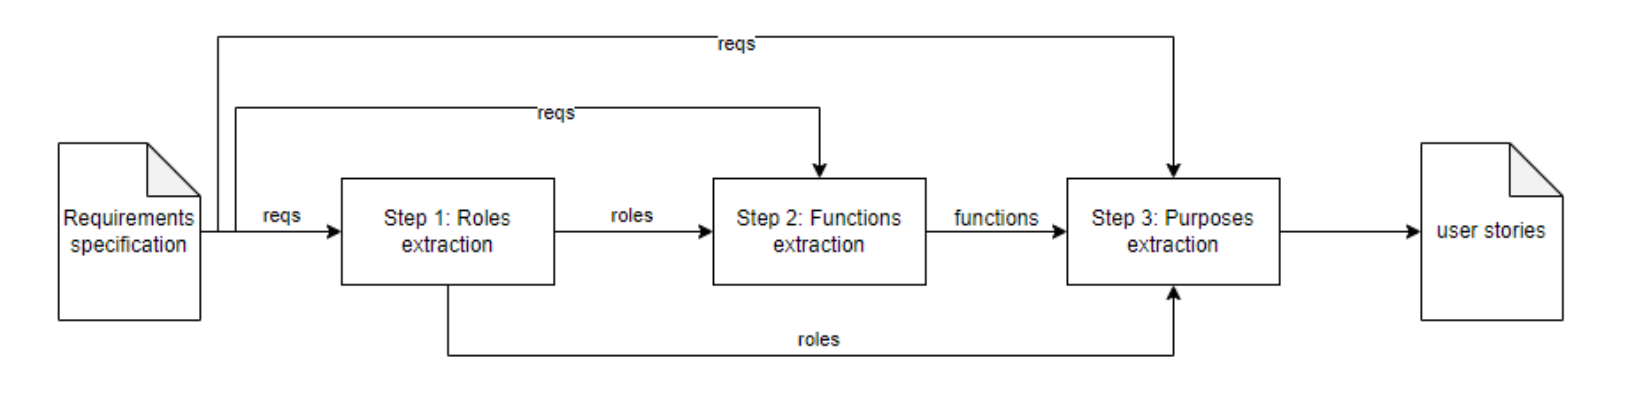
\includegraphics[width=\linewidth]{../../../lab07/architecture_diagram.png}\caption{Notebook-provided architecture: requirements feed role extraction, then functions and purposes, producing user stories.}\label{fig:lab07-architecture}\end{figure}

\subsection{Model setup and prompt serialization}

\medskip\noindent The pipeline begins with a fixed seed, the available compute device, and Llama 3.2 3B Instruct loaded from the locally authenticated Hugging Face account. The helper accepts chat-template prompts, avoids adding a second BOS token, samples at temperature 0.15, and stops at either Llama's end-of-turn or EOS token. After decoding, it frees generated tensors and clears the MPS cache. These shared settings apply to role, function, and purpose generation.
% coverage-cell: LABS/lab07/text-07-stories.ipynb cell=0 source_sha256=ff72705d448129199faede751830b17add7ee35634a1b529debe8205658f146c
\begin{lstlisting}[style=studycode]
# ------------------ Initial setup ---------------------
import gc
import torch
from huggingface_hub import get_token
from transformers import AutoTokenizer, AutoModelForCausalLM, set_seed

set_seed(42)
torch.set_num_threads(2)
device = torch.device("cuda" if torch.cuda.is_available() else "mps" if torch.backends.mps.is_available() else "cpu")
print("Using device:", device)

# Read a local saved login or HF_TOKEN; never store a token in the notebook.
hf_token = get_token()
model_id = "meta-llama/Llama-3.2-3B-Instruct"
model = AutoModelForCausalLM.from_pretrained(
    model_id, torch_dtype=torch.float16, low_cpu_mem_usage=True, token=hf_token,
).to(device).eval()
tokenizer = AutoTokenizer.from_pretrained(model_id, token=hf_token, clean_up_tokenization_spaces=False)
tokenizer.pad_token = tokenizer.eos_token


def make_a_query(prompt: str, tokenizer, model, device, max_new_tokens: int = 200):
    # Chat-template prompts already contain special tokens; do not add another BOS.
    inputs = tokenizer(prompt, return_tensors="pt", add_special_tokens=False).to(device)
    prompt_length = inputs["input_ids"].shape[1]
    eot_id = tokenizer.convert_tokens_to_ids("<|eot_id|>")
    with torch.inference_mode():
        output = model.generate(
            **inputs,
            max_new_tokens=max_new_tokens,
            do_sample=True,
            temperature=0.15,
            top_p=0.9,
            num_beams=1,
            # Stop on Llama's end-of-turn marker and the model's EOS marker.
            eos_token_id=list(dict.fromkeys([eot_id, tokenizer.eos_token_id])),
            pad_token_id=tokenizer.pad_token_id,
        )
    answer = tokenizer.decode(output[0, prompt_length:], skip_special_tokens=True).strip()
    del output, inputs
    gc.collect()
    if getattr(device, "type", str(device)) == "mps":
        torch.mps.empty_cache()
    return answer
\end{lstlisting}
\par\smallskip
% coverage-output: LABS/lab07/text-07-stories.ipynb cell=0 output=0 source_sha256=ff72705d448129199faede751830b17add7ee35634a1b529debe8205658f146c payload_sha256=847a6378f797e9761a715ffe0c45802bb4f5f8f1f6bb33ca9aa4a90e966d7abe artifact=study_guide/execution_artifacts/lab07/lab07/text-07-stories_cell_0000_ff72705d4481_output_0.txt
\label{out:lab07-stories-0000-00}
\lstinputlisting[style=terminalOutput]{../../execution_artifacts/lab07/lab07/text-07-stories_cell_0000_ff72705d4481_output_0.txt}
% coverage-output: LABS/lab07/text-07-stories.ipynb cell=0 output=1 source_sha256=ff72705d448129199faede751830b17add7ee35634a1b529debe8205658f146c payload_sha256=b41efeece60cddf239ffc076476f5b040c0c482e4748d1045be6be5a9ef70b2d artifact=study_guide/execution_artifacts/lab07/lab07/text-07-stories_cell_0000_ff72705d4481_output_1.txt
\label{out:lab07-stories-0000-01}
\lstinputlisting[style=terminalOutput]{../../execution_artifacts/lab07/lab07/text-07-stories_cell_0000_ff72705d4481_output_1.txt}
% coverage-output: LABS/lab07/text-07-stories.ipynb cell=0 output=2 source_sha256=ff72705d448129199faede751830b17add7ee35634a1b529debe8205658f146c payload_sha256=fa52eeb332a913bde139573dd57f4c07ecd15b7fb5674d04824f0776fd330e88 artifact=study_guide/execution_artifacts/lab07/lab07/text-07-stories_cell_0000_ff72705d4481_output_2.txt
\label{out:lab07-stories-0000-02}
\lstinputlisting[style=terminalOutput]{../../execution_artifacts/lab07/lab07/text-07-stories_cell_0000_ff72705d4481_output_2.txt}
% coverage-output: LABS/lab07/text-07-stories.ipynb cell=0 output=3 source_sha256=ff72705d448129199faede751830b17add7ee35634a1b529debe8205658f146c payload_sha256=e74f9d108e5a7f103153a1aa0b0a57602db93582d4d57be1c469fd20a7c4679c artifact=study_guide/execution_artifacts/lab07/lab07/text-07-stories_cell_0000_ff72705d4481_output_3.txt
\label{out:lab07-stories-0000-03}
\lstinputlisting[style=terminalOutput]{../../execution_artifacts/lab07/lab07/text-07-stories_cell_0000_ff72705d4481_output_3.txt}
% coverage-output: LABS/lab07/text-07-stories.ipynb cell=0 output=4 source_sha256=ff72705d448129199faede751830b17add7ee35634a1b529debe8205658f146c payload_sha256=baba98f033973646129c2263926af02ea52be9867186013fa3924651a7f00181 artifact=study_guide/execution_artifacts/lab07/lab07/text-07-stories_cell_0000_ff72705d4481_output_4.txt
\label{out:lab07-stories-0000-04}
\lstinputlisting[style=terminalOutput]{../../execution_artifacts/lab07/lab07/text-07-stories_cell_0000_ff72705d4481_output_4.txt}
% coverage-output: LABS/lab07/text-07-stories.ipynb cell=0 output=5 source_sha256=ff72705d448129199faede751830b17add7ee35634a1b529debe8205658f146c payload_sha256=9fd3b0e5381587fe64627eebf5b8b04bde395ee0abca18f217a081a1e5ab04af artifact=study_guide/execution_artifacts/lab07/lab07/text-07-stories_cell_0000_ff72705d4481_output_5.txt
\label{out:lab07-stories-0000-05}
\lstinputlisting[style=terminalOutput]{../../execution_artifacts/lab07/lab07/text-07-stories_cell_0000_ff72705d4481_output_5.txt}
% coverage-output: LABS/lab07/text-07-stories.ipynb cell=0 output=6 source_sha256=ff72705d448129199faede751830b17add7ee35634a1b529debe8205658f146c payload_sha256=20edaa3e50bf40ea9d7f0ac1fb0c44b3e7771949761d7a46df51f9ab1ceac876 artifact=-
\label{out:lab07-stories-0000-06}
\textit{This notebook output has no printable text representation.}
The output confirms MPS selection and successful model initialization; the loading progress and library warnings are execution diagnostics rather than model answers. Authentication comes from the local Hugging Face credential store, never the notebook. The checkpoint is loaded in FP16. The environment and model revision accompany the run record for reproducibility.

\medskip\noindent The requirements specification is the shared input for all later stages. Before extracting stories, this cell contrasts a manually serialized system/user conversation with the tokenizer's official chat-template serializer using a small capital-city question. The demo isolates prompt structure from the hiking requirements and shows how an assistant-generation prefix is formed.
% coverage-cell: LABS/lab07/text-07-stories.ipynb cell=2 source_sha256=dcee2b7c138d7ddb33002e041be56790a0b7c4e6b1eb7b9ae4e173896bb40656
\begin{lstlisting}[style=studycode]
#reference requirements_text

requirements_text = "The proposed platform is designed to enhance the hiking experience for various user groups, including visitors, local guides, platform managers, and hut workers. The platform provides a centralized repository of hiking routes, hut information, and parking facilities. It also enables interactive features such as real-time hike tracking, personalized recommendations, and group hike planning. By combining these capabilities, the platform seeks to foster safe, informed, and collaborative hiking experiences.\
The platform will be deployed as a cloud-based web and mobile application accessible to all stakeholders. The distribution strategy includes an app available on major mobile operating systems, such as iOS and Android, alongside a responsive web interface. It will require an internet connection for features like real-time tracking, notifications, and user authentication, though some offline capabilities, such as pre-downloaded hike information, will also be available.\
User authentication will be role-based, ensuring that only authorized users, such as verified hut workers and platform managers, can access sensitive or administrative features.\
Visitors are the primary users of the platform. They can browse a comprehensive list of hiking trails, filter them based on specific criteria such as difficulty, length, or starting point, and view detailed descriptions. To access advanced features like personalized recommendations, visitors can create user accounts by registering on the platform. Registered users can record their fitness parameters, enabling the system to suggest trails tailored to their capabilities.\
During a hike, visitors can record their progress by marking reference points and sharing their live location through a broadcasting URL. They can also initiate group activities by planning hikes, adding group members, and confirming group participation. The platform allows visitors to start, terminate, and track their hikes, with notifications for unfinished hikes or late group members to ensure safety and accountability.\
Local guides enrich the platform by contributing essential information. They can add detailed descriptions of hikes, parking facilities, and huts, ensuring hikers have accurate and comprehensive data. Local guides also link parking lots and huts to specific trails as starting or arrival points, enhancing the planning process.\
To aid in the visual representation and accessibility of information, local guides can upload pictures of huts and connect these locations directly to hikes. This integration simplifies route planning and helps visitors visualize their journey.\
Platform managers oversee the operational integrity and safety of the platform. They verify new hut worker registrations, ensuring that only authorized personnel can update hut-related data. Managers can also broadcast weather alerts for specific areas, notifying all hikers in those regions through push notifications. This ensures that users stay informed about potentially hazardous conditions.\
The platform manager's role includes maintaining an organized and secure user system while facilitating collaboration between local guides, hut workers, and visitors.\
Hut workers are critical to the maintenance of up-to-date trail and accommodation information. After registering and being verified, hut workers can log into the platform to add or update information about their assigned huts, including uploading pictures and describing the facilities available. They can also monitor and report on the condition of nearby trails, ensuring hikers receive current information.\
Hut workers play a vital role in providing situational updates for hikers. For instance, if a nearby trail is impacted by severe weather or physical obstructions, they can communicate these conditions through the platform. This enhances the safety and preparedness of all hikers relying on the platform."


#---------------------Example usage - without chat template and customized system prompt------------------
prompt = """<|begin_of_text|><|start_header_id|>system<|end_header_id|>

You are an expert on world capitals.
Respond with only the capital city of the given country. Do not repeat the question.<|eot_id|>
<|start_header_id|>user<|end_header_id|>

What is the capital of France?<|eot_id|>
<|start_header_id|>assistant<|end_header_id|>

"""

response = make_a_query(prompt, tokenizer, model, device)

print(f"Prompt: {prompt}\n\nResponse: {response}")
#----------------------------------------------------------------------------


#---------------------Example usage - with chat template and customized system prompt---------------------
messages = [
    {"role": "system", "content": "You are an expert on world capitals. Respond with only the capital city of the given country. Do not repeat the question."},
    {"role": "user", "content": "What is the capital of France?"}
]

chat = tokenizer.apply_chat_template(messages,
                                     tokenize=False, #IMPORTANT: only the special tokens are added, we'll apply tokenisation later
                                     add_generation_prompt=True) # adds the placeholder for the assistant's response


response = make_a_query(chat, tokenizer, model, device)

print("------------------------------------------------------------")
print(f"Prompt: {chat}\n\nResponse: {response}")
\end{lstlisting}
\par\smallskip
% coverage-output: LABS/lab07/text-07-stories.ipynb cell=2 output=0 source_sha256=dcee2b7c138d7ddb33002e041be56790a0b7c4e6b1eb7b9ae4e173896bb40656 payload_sha256=18573567b0a435b1addf53e49b09480b0978ab729bca047c7a5735be717f2464 artifact=study_guide/execution_artifacts/lab07/lab07/text-07-stories_cell_0002_dcee2b7c138d_output_0.txt
\label{out:lab07-stories-0002-00}
\lstinputlisting[style=terminalOutput]{../../execution_artifacts/lab07/lab07/text-07-stories_cell_0002_dcee2b7c138d_output_0.txt}
% coverage-output: LABS/lab07/text-07-stories.ipynb cell=2 output=1 source_sha256=dcee2b7c138d7ddb33002e041be56790a0b7c4e6b1eb7b9ae4e173896bb40656 payload_sha256=f183802cc1037cee48e0a190cc6a83c143dfe6cfaacca18f0e4910c0b70745d2 artifact=study_guide/execution_artifacts/lab07/lab07/text-07-stories_cell_0002_dcee2b7c138d_output_1.txt
\label{out:lab07-stories-0002-01}
\lstinputlisting[style=terminalOutput]{../../execution_artifacts/lab07/lab07/text-07-stories_cell_0002_dcee2b7c138d_output_1.txt}
Both paths return exactly \texttt{Paris}. The manual serialization visibly supplies its own system and user headers, while the tokenizer-generated template inserts the model's system metadata (knowledge-cutoff and current date) before the same messages. Both include an assistant-generation prefix; using the official template prevents hand-written header mistakes. Because the prompt text already includes the serialized tokens, \texttt{add\_special\_tokens=False} in the shared helper avoids adding a second beginning token.

\subsection{Extracting and evaluating roles}

The first extraction stage asks the same model to identify the people and stakeholders represented in the hiking-platform requirements. The prompts below differ only in their in-context examples; the CSV reference is prepared separately so the scoring target does not depend on the generated response.

\medskip\noindent This cell creates zero-shot, one-shot, and few-shot role-extraction prompts. The one-shot and few-shot examples are represented as complete alternating user/assistant messages, so each demonstration teaches both the task and the requested list format. The same hiking requirements are then appended as the final user query to each prompt.
% coverage-cell: LABS/lab07/text-07-stories.ipynb cell=4 source_sha256=b11ebf08ba13a699332444406302e478d2420ef31c808a819090ac4e8668b83f
\begin{lstlisting}[style=studycode]
#define three different prompts for extracting users, using the zero-shot, one-shot and few-shot approach. then evaluate the difference in terms of capability to format the output and actual results

# IMPORTANT: wheter you use the chat template or not, remember to add the shots into the correct structure composed by user's query and assistant's response (see previous lab)

query = "Requirements Text:\n" + requirements_text + "\nList the distinct user roles."

shots = [ # This is a list of lists, useful to separate each shot from each other

    # First shot
    [
        {'role': 'user',
          'content': """Requirements Text:
"The application is designed to streamline food delivery operations. Customers can browse menus and place orders. Delivery personnel use the app to view delivery assignments and update order statuses. Restaurant managers can manage their menus and track incoming orders."""},
        {'role': 'assistant', 'content': """1. Customers
2. Delivery Personnel
3. Restaurant Managers"""},
    ],

    # Second shot
    [
      {'role': 'user',
      'content': """Requirements Text:
The platform supports the education sector by providing tools for students, teachers, and administrators. Students can access course materials, submit assignments, and track their progress. Teachers can create content, grade submissions, and communicate with students. Administrators oversee user registrations and system performance."""},
      {'role': 'assistant',
      'content': """1. Students
2. Teachers
3. Administrators"""}
    ],

    # Third shot
    [
        {'role': 'user',
         'content': """Requirements Text:
The system provides real-time updates for commuters, transit operators, and city planners. Commuters can check schedules and delays. Transit operators monitor vehicle statuses and manage timetables. City planners analyze system data to improve routes and infrastructure."""},
        {'role': 'assistant',
         'content': """1. Commuters
2. Transit Operators
3. City Planners"""}
    ]
]


system_prompt = """Extract only the distinct user roles explicitly supported by the supplied requirements.
Return only the role names explicitly stated in the requirements, one per numbered line in the form `1. Role name`.
Do not include a heading, introduction, rationale, examples, actions, or commentary.
Stop immediately after the final role. Do not infer roles absent from the text."""

# Build the message list for each promoting technique

messages_zero_shot = [{"role": "system", "content": system_prompt}, {"role": "user", "content": query}]
prompt_zero_shot = tokenizer.apply_chat_template(messages_zero_shot, tokenize=False, add_generation_prompt=True)

messages_one_shot = [{"role": "system", "content": system_prompt}] + shots[0] + [{"role": "user", "content": query}]
prompt_one_shot = tokenizer.apply_chat_template(messages_one_shot, tokenize=False, add_generation_prompt=True)

messages_few_shots = [{"role": "system", "content": system_prompt}] + [message for shot in shots for message in shot] + [{"role": "user", "content": query}]
prompt_few_shots = tokenizer.apply_chat_template(messages_few_shots, tokenize=False, add_generation_prompt=True)


# Call the LLM function for the three prompts and print the results
roles_extracted_zero_shot = make_a_query(prompt_zero_shot, tokenizer, model, device, max_new_tokens=96)

print("Extracted Roles - zero shot: \n", roles_extracted_zero_shot)

roles_extracted_one_shot = make_a_query(prompt_one_shot, tokenizer, model, device, max_new_tokens=96)

print("Extracted Roles - one shot: \n", roles_extracted_one_shot)


roles_extracted_few_shots = make_a_query(prompt_few_shots, tokenizer, model, device, max_new_tokens=96)

print("Extracted Roles - few shots: \n", roles_extracted_few_shots)
\end{lstlisting}
\par\smallskip
% coverage-output: LABS/lab07/text-07-stories.ipynb cell=4 output=0 source_sha256=b11ebf08ba13a699332444406302e478d2420ef31c808a819090ac4e8668b83f payload_sha256=b1541258829777bf2b48241201d7ef3eefbc75a50f8fe2f3ad545ca0674256f2 artifact=study_guide/execution_artifacts/lab07/lab07/text-07-stories_cell_0004_b11ebf08ba13_output_0.txt
\label{out:lab07-stories-0004-00}
\lstinputlisting[style=terminalOutput]{../../execution_artifacts/lab07/lab07/text-07-stories_cell_0004_b11ebf08ba13_output_0.txt}
% coverage-output: LABS/lab07/text-07-stories.ipynb cell=4 output=1 source_sha256=b11ebf08ba13a699332444406302e478d2420ef31c808a819090ac4e8668b83f payload_sha256=924a363f71ca47f04757d67a88972d0b47d5ed98d5a7878b334254fb011a80a5 artifact=study_guide/execution_artifacts/lab07/lab07/text-07-stories_cell_0004_b11ebf08ba13_output_1.txt
\label{out:lab07-stories-0004-01}
\lstinputlisting[style=terminalOutput]{../../execution_artifacts/lab07/lab07/text-07-stories_cell_0004_b11ebf08ba13_output_1.txt}
% coverage-output: LABS/lab07/text-07-stories.ipynb cell=4 output=2 source_sha256=b11ebf08ba13a699332444406302e478d2420ef31c808a819090ac4e8668b83f payload_sha256=a1046c427bc65d55f9d9875694d92f34f619dcc6dba6fb7d6c7b45f18695aba1 artifact=study_guide/execution_artifacts/lab07/lab07/text-07-stories_cell_0004_b11ebf08ba13_output_2.txt
\label{out:lab07-stories-0004-02}
\lstinputlisting[style=terminalOutput]{../../execution_artifacts/lab07/lab07/text-07-stories_cell_0004_b11ebf08ba13_output_2.txt}
All three prompt conditions returned the same four roles: visitors, local guides, platform managers, and hut workers. The consistency is useful, but the CSV comparison later shows the list misses two reference roles. In this recorded run, adding demonstrations did not change the extracted list; format compliance should not be confused with full coverage.

\medskip\noindent The evaluation reference is derived from the supplied \texttt{stories.csv}. The helper scans each user-story description for its 'As a ... I want' role phrase, removes duplicates, and sorts the result. Keeping reference preparation in its own cell makes it possible to audit the target set independently of the language model.
% coverage-cell: LABS/lab07/text-07-stories.ipynb cell=6 source_sha256=4aa3588c78580c37180c2ae11f3104e64c4f14bf82c16b2b01f4047d58d8553c
\begin{lstlisting}[style=studycode]
import csv
import re


def extract_unique_roles(file_path: str):
    roles = set()
    with open(file_path, newline="", encoding="utf-8-sig") as stream:
        for row in csv.DictReader(stream):
            match = re.search(r"^As\s+(?:an?\s+)?(.+?)\s+I\s+want\b", row["Description"].strip(), flags=re.IGNORECASE)
            if match:
                roles.add(match.group(1).strip().lower())
    return sorted(roles)


def extract_list_items(text: str):
    """Keep only a leading numbered/bulleted list; reject explanatory prose."""
    items = []
    started = False
    for line in text.splitlines():
        line = line.strip()
        match = re.match(r"^(?:\d+\s*[.)-]?\s+|[-*•]\s+)(.+?)\s*$", line)
        if match:
            started = True
            item = match.group(1).strip().strip("* ")
            # Keep the role label and discard parenthetical/editorial commentary.
            item = re.split(r"\s+[–—]\s+|\s+-\s+", item, maxsplit=1)[0]
            item = re.sub(r"\s*\([^)]*\)", "", item).strip()
            item = re.sub(r"/s$", "s", item, flags=re.IGNORECASE)
            if item:
                items.append(item)
        elif started and line:
            break
    return list(dict.fromkeys(items))


def normalize_roles(role_list: list[str]):
    # Ignore whitespace, case and a final plural s as requested by the exercise.
    return {re.sub(r"\s+", "", role.lower()).removesuffix("s") for role in role_list if role.strip()}


def role_metrics(expected, actual):
    expected, actual = normalize_roles(expected), normalize_roles(actual)
    tp = len(expected & actual)
    fp = len(actual - expected)
    fn = len(expected - actual)
    return tp, fp, fn, tp / (tp + fp) if tp + fp else 0.0, tp / (tp + fn) if tp + fn else 0.0


file_path = "stories.csv"
expected_roles = extract_unique_roles(file_path)
print("Reference roles from stories.csv:", expected_roles)
\end{lstlisting}
\par\smallskip
% coverage-output: LABS/lab07/text-07-stories.ipynb cell=6 output=0 source_sha256=4aa3588c78580c37180c2ae11f3104e64c4f14bf82c16b2b01f4047d58d8553c payload_sha256=a16faa4b0ea6c40de05aabdf9e0c61dc3507275b316a39e428ba1de5dc15c7cb artifact=study_guide/execution_artifacts/lab07/lab07/text-07-stories_cell_0006_4aa3588c7858_output_0.txt
\label{out:lab07-stories-0006-00}
\lstinputlisting[style=terminalOutput]{../../execution_artifacts/lab07/lab07/text-07-stories_cell_0006_4aa3588c7858_output_0.txt}
The printed set contains the six distinct role phrases extracted from the CSV. The parenthetical phrase in the first description is retained as part of its role string; the following normalization handles case, whitespace, and a final plural 's', but does not semantically rewrite role names.

\medskip\noindent This cell parses the few-shot model answer into list items, normalizes the extracted and reference roles, and counts true positives, false positives, and false negatives. Precision is the fraction of extracted roles that match the reference; recall is the fraction of reference roles recovered. The formulas return zero when their denominator is empty, avoiding a division error for empty sets.
% coverage-cell: LABS/lab07/text-07-stories.ipynb cell=7 source_sha256=c90bb51175b30d8a6ddd5f7a02266d6837669894e45ab654f595930d061ac97f
\begin{lstlisting}[style=studycode]
actual_roles = extract_list_items(roles_extracted_few_shots)
print("Roles extracted by the model:", actual_roles)
true_positives, false_positives, false_negatives, precision, recall = role_metrics(expected_roles, actual_roles)
print("True Positives:", true_positives)
print("False Positives:", false_positives)
print("False Negatives:", false_negatives)
print("Precision:", precision)
print("Recall:", recall)
\end{lstlisting}
\par\smallskip
% coverage-output: LABS/lab07/text-07-stories.ipynb cell=7 output=0 source_sha256=c90bb51175b30d8a6ddd5f7a02266d6837669894e45ab654f595930d061ac97f payload_sha256=e816067f86a86f6da2fc08cf6ab7b9f1965b8ebc9d859c0b470a4206eb14abeb artifact=study_guide/execution_artifacts/lab07/lab07/text-07-stories_cell_0007_c90bb51175b3_output_0.txt
\label{out:lab07-stories-0007-00}
\lstinputlisting[style=terminalOutput]{../../execution_artifacts/lab07/lab07/text-07-stories_cell_0007_c90bb51175b3_output_0.txt}
The run reports four true positives, zero false positives, and two false negatives. Precision is 1.0 because every extracted role appears in the CSV reference; recall is 0.667 because two CSV roles were missed. These scores reflect this reference and exact string normalization; they do not establish semantic equivalence or measure zero-shot and one-shot answers, which happen to match in this run.

\subsection{From roles to functions and purposes}

Role names narrow the next prompt to actions that a stakeholder needs from the platform. The notebook converts each extracted action into a provisional role/function story, then asks for the reason behind one such action to complete the familiar 'As a ..., I want ..., so that ...' form.

\medskip\noindent For each extracted role, this loop asks for concise actions grounded in the complete hiking requirements. A food-delivery example demonstrates the expected numbered-list shape, while the actual query includes the full requirements and names the current role. The parser accepts only an initial, contiguous numbered or bulleted list; it skips a response that begins with NONE or prose, and stops at commentary. Accepted actions become provisional 'As a role, I want to function' tuples.
% coverage-cell: LABS/lab07/text-07-stories.ipynb cell=9 source_sha256=ff9552db17b0693deeb4bac390c32031c36a4a26cc7e5cbde43cf8617cdd487d
\begin{lstlisting}[style=studycode]
current_roles = actual_roles
user_stories = list()

#this function will be used to extract the functions from the answer provided by the llm agent

def extract_functions(text: str):
    """Accept only an initial, contiguous numbered/bulleted list of functions."""
    functions = []
    started = False
    for line in text.splitlines():
        line = line.strip()
        if not line:
            if started:
                break
            continue
        if line.upper() == "NONE":
            return []
        match = re.match(r"^(?:\d+[.)]|[-*•])\s+(.+?)\s*$", line)
        if not match:
            if started:
                break
            return []
        started = True
        item = match.group(1).strip().rstrip(".")
        if item:
            functions.append(item)
    return list(dict.fromkeys(functions))



#this function can be used to format a user story in the expected format. it returns a list of tuples (user, story)

def create_user_stories(role: str, functions: list[str]):
    """
    Generate user stories in the standard format.
    """
    user_stories = [(role, f"As a {role}, I want to {function}") for function in functions]
    return user_stories


for role in current_roles:

    #1. Loop over the list of roles and extract the piece of text from requirements related to that role
    print("\n\nExtracting stories for role", role)


    #define a prompt to extract functions for a given user
    #the prompt will be composed of the following fields:
    # - context: usage persona of the Lllama agent and instructions
    # - examples: examples of requirements text, role and user
    # - task: description of the task to perform. here you have to provide the current role
    # - answer field: placeholder from which the response will start

    #a tentative example can be the following one (you can generate many of them for instance by using another LLM agent, e.g. ChatGPT)
    example_text = [
        {
            'role': 'user',
            'content': """**Requirements Text**:
The application is designed to streamline food delivery operations. Customers can browse menus and place orders. Delivery personnel use the app to view delivery assignments and update order statuses. Restaurant managers can manage their menus and track incoming orders.

Role: Delivery personnel
List the functions for this role."""
        },

        {
            'role': 'assistant',
            'content': """1. View delivery assignments.
2. Update order status."""
        }
    ]

    system_prompt = (
        "Extract only actions explicitly supported by the requirements for the requested role. "
        "Return 1 to 8 numbered lines, each formatted `1. Verb phrase` and no more than eight words. "
        "Use no heading, explanation, prose, claims, or action not stated in the requirements. "
        "Stop after the final list item. If no action is stated for that role, return exactly `NONE`."
    )

    query = f"Requirements Text:\n{requirements_text}\n\nRole: {role}\nList the functions for this role."

    messages = [{"role": "system", "content": system_prompt}] + example_text + [{"role": "user", "content": query}]
    prompt = tokenizer.apply_chat_template(messages, tokenize=False, add_generation_prompt=True)


    #now ask the agent and get the response
    response = make_a_query(prompt, tokenizer, model, device, max_new_tokens=128)  # Memory-safe cap for a concise numbered action list

    print(response)

    functions = extract_functions(response)

    tmp_user_stories = create_user_stories(role, functions)
    if not functions:
        if response.strip().upper() == "NONE":
            print("No explicit supported functions were returned for this role.")
            continue
        raise ValueError(f"The model returned no numbered functions for {role}: {response}")
    user_stories.extend(tmp_user_stories)
\end{lstlisting}
\par\smallskip
% coverage-output: LABS/lab07/text-07-stories.ipynb cell=9 output=0 source_sha256=ff9552db17b0693deeb4bac390c32031c36a4a26cc7e5cbde43cf8617cdd487d payload_sha256=8dd2b367147b8dc78a008860a53bd2ab93a6da1b43ddcba01327deccb917fcae artifact=study_guide/execution_artifacts/lab07/lab07/text-07-stories_cell_0009_ff9552db17b0_output_0.txt
\label{out:lab07-stories-0009-00}
\lstinputlisting[style=terminalOutput]{../../execution_artifacts/lab07/lab07/text-07-stories_cell_0009_ff9552db17b0_output_0.txt}
% coverage-output: LABS/lab07/text-07-stories.ipynb cell=9 output=1 source_sha256=ff9552db17b0693deeb4bac390c32031c36a4a26cc7e5cbde43cf8617cdd487d payload_sha256=92b8153f71914cd1bbdbd76cfd70cd66b141511d232c99d5530df38736544642 artifact=study_guide/execution_artifacts/lab07/lab07/text-07-stories_cell_0009_ff9552db17b0_output_1.txt
\label{out:lab07-stories-0009-01}
\lstinputlisting[style=terminalOutput]{../../execution_artifacts/lab07/lab07/text-07-stories_cell_0009_ff9552db17b0_output_1.txt}
% coverage-output: LABS/lab07/text-07-stories.ipynb cell=9 output=2 source_sha256=ff9552db17b0693deeb4bac390c32031c36a4a26cc7e5cbde43cf8617cdd487d payload_sha256=3dd5842e2454c30976714cb83f281416c68116c6eeda97d8ece55093445f0aa3 artifact=study_guide/execution_artifacts/lab07/lab07/text-07-stories_cell_0009_ff9552db17b0_output_2.txt
\label{out:lab07-stories-0009-02}
\lstinputlisting[style=terminalOutput]{../../execution_artifacts/lab07/lab07/text-07-stories_cell_0009_ff9552db17b0_output_2.txt}
% coverage-output: LABS/lab07/text-07-stories.ipynb cell=9 output=3 source_sha256=ff9552db17b0693deeb4bac390c32031c36a4a26cc7e5cbde43cf8617cdd487d payload_sha256=cb3343a5ae691c9bc58824084da1ac592a4a82c834603210882f255d6cd1abfb artifact=study_guide/execution_artifacts/lab07/lab07/text-07-stories_cell_0009_ff9552db17b0_output_3.txt
\label{out:lab07-stories-0009-03}
\lstinputlisting[style=terminalOutput]{../../execution_artifacts/lab07/lab07/text-07-stories_cell_0009_ff9552db17b0_output_3.txt}
% coverage-output: LABS/lab07/text-07-stories.ipynb cell=9 output=4 source_sha256=ff9552db17b0693deeb4bac390c32031c36a4a26cc7e5cbde43cf8617cdd487d payload_sha256=a98100a8721f005733a80808b4a944e5e9c5f555b4ce609f1eaadfbfa366496a artifact=study_guide/execution_artifacts/lab07/lab07/text-07-stories_cell_0009_ff9552db17b0_output_4.txt
\label{out:lab07-stories-0009-04}
\lstinputlisting[style=terminalOutput]{../../execution_artifacts/lab07/lab07/text-07-stories_cell_0009_ff9552db17b0_output_4.txt}
The recorded run returns numbered functions for all four extracted roles. The actions are relevant paraphrases of the requirements, not an independently verified or exhaustive inventory. Importantly, no per-role requirement excerpt is constructed despite the original comments describing that as an option; each prompt receives the full requirements.

\medskip\noindent The final cell demonstrates the 'so that' step for the first generated role/function pair. It separates the existing role and function from the provisional story, then asks the model to infer one purpose using the original requirements and a single worked example. This cell demonstrates purpose generation for one pair rather than completing every tuple in the collection.
% coverage-cell: LABS/lab07/text-07-stories.ipynb cell=11 source_sha256=5e5466de46af074a357fa29c81e6b66506322daa27db854d43871031e8cb95ed
\begin{lstlisting}[style=studycode]
# Demonstrate purpose extraction for one (role, story) pair, as requested.
if not user_stories:
    raise ValueError("No user stories were generated in the previous step.")
user_story1 = user_stories[0]
role, initial_story = user_story1
prefix = f"As a {role}, I want to "
function = initial_story[len(prefix):] if initial_story.startswith(prefix) else initial_story
print("Role:", role)
print("Function:", function)

system_prompt = (
    "You are a requirements analyst. Use the requirements and the given role and function "
    "to infer the supported purpose. Return exactly one complete story in the format "
    "'As a <role>, I want to <function>, so that <purpose>.' Do not invent capabilities "
    "or add an explanation."
)
shot_examples = [
    {"role": "user", "content": "Requirements: Visitors filter hiking trails by difficulty, length, or starting point to select a suitable route.\nRole: visitor\nFunction: filter hiking trails by difficulty"},
    {"role": "assistant", "content": "As a visitor, I want to filter hiking trails by difficulty, so that I can choose a route suited to my abilities."},
]
query = f"Requirements:\n{requirements_text}\n\nRole: {role}\nFunction: {function}"
messages = [{"role": "system", "content": system_prompt}] + shot_examples + [{"role": "user", "content": query}]
prompt = tokenizer.apply_chat_template(messages, tokenize=False, add_generation_prompt=True)
response = make_a_query(prompt, tokenizer, model, device, max_new_tokens=128)  # One concise user-story purpose clause
print(response)
\end{lstlisting}
\par\smallskip
% coverage-output: LABS/lab07/text-07-stories.ipynb cell=11 output=0 source_sha256=5e5466de46af074a357fa29c81e6b66506322daa27db854d43871031e8cb95ed payload_sha256=9c01567c2a705b3b7e811639f8444d93bda78afafe02710b9034f5904545146f artifact=study_guide/execution_artifacts/lab07/lab07/text-07-stories_cell_0011_5e5466de46af_output_0.txt
\label{out:lab07-stories-0011-00}
\lstinputlisting[style=terminalOutput]{../../execution_artifacts/lab07/lab07/text-07-stories_cell_0011_5e5466de46af_output_0.txt}
% coverage-output: LABS/lab07/text-07-stories.ipynb cell=11 output=1 source_sha256=5e5466de46af074a357fa29c81e6b66506322daa27db854d43871031e8cb95ed payload_sha256=4329b5529d347784c3ad87431f6fabb100ed3ca290a5e247bdbc2cf8b1dc422c artifact=study_guide/execution_artifacts/lab07/lab07/text-07-stories_cell_0011_5e5466de46af_output_1.txt
\label{out:lab07-stories-0011-01}
\lstinputlisting[style=terminalOutput]{../../execution_artifacts/lab07/lab07/text-07-stories_cell_0011_5e5466de46af_output_1.txt}
The printed role and function identify the first tuple, and the response demonstrates one 'so that' completion: exploring and discovering suitable hiking routes. The revised in-context example now uses hiking preferences and abilities rather than an unrelated domain. This final cell handles only one pair, so it neither completes all tuples nor validates every earlier function.

\begin{quote}\textbf{Reading the result.} The exercise demonstrates a staged requirements-analysis workflow and a simple reference-based metric. Its final purpose-generation cell handles only the first role/function pair, and automatic extraction can omit, duplicate, or paraphrase requirements. A human review is still needed before treating generated stories as accepted requirements.\end{quote}

\section{Execution and reproducibility notes}

The matching lecture recording was not available in Whisper or in the supplied course files during this run. Per the task scope, lecture review is deferred until the professor provides the recordings; explanations here are based on the notebook's assignment text, source, provided architecture image, and saved outputs.

The model is \texttt{meta-llama/Llama-3.2-3B-Instruct}, loaded in FP16 on MPS from the locally authenticated Hugging Face account. Generation uses seeded low-temperature sampling with one beam and task-specific token caps. Samples can vary across framework versions, kernels, and model revisions. The exact dependency versions, model revision, and execution records are listed in the accompanying environment and provenance files.

\end{document}

\end{document}
